\section{"Interaction naturelle" et rehabilitation}

\subsection{Applications orientés "fitness"}

\subsubsection{Wii Fit}

Si certains jeu proposaient déjà une interaction naturelle, avec l'EyeToy 
de la Playstation de Sony (2003), la console Wii de Nintendo (2006) est 
l'amorce claire de l'enthousiasme présent vis-à-vis de telles interfaces, et cet enthousiasme va bien
au delà des jeux. 
Si nous avons aujourd'hui la Kinect de Microsoft ou encore la
PS Eye de Sony, c'est grâce à son controleur (voir figure~\ref{fig:wii}), 
capable de reconnaître des mouvement à 
travers l'espace grâce à un système d'accéléromètres. 

\begin{figure}[h!]
\centering
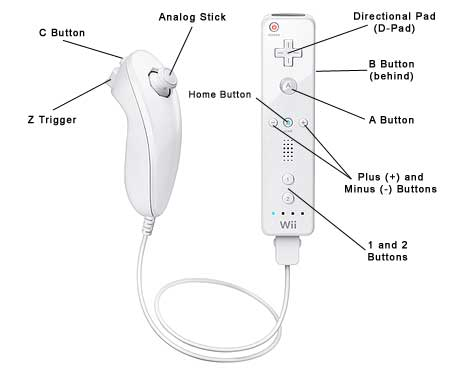
\includegraphics[width=0.7\linewidth]{images/wii_diagram}
\caption{Le controleur de la console Wii de Nintendo.}
\label{fig:wii}
\end{figure}

Avec le jeu Wii Fit, Nintendo ajoute la Wii Balance Board (voir figure 
\ref{fig:balance_board}). C'est une accessoire capable de mesurer le 
poids mis sur chaque pied et donc la position du centre de masse. Quant au jeu,
il propose un suivie de la mise en forme du joueur à travers des graphiques, 
points et barres de progression\ref{fig:wii_fit}~: de la "gamification", 
tout simplement.

\begin{figure}[h!]
\centering
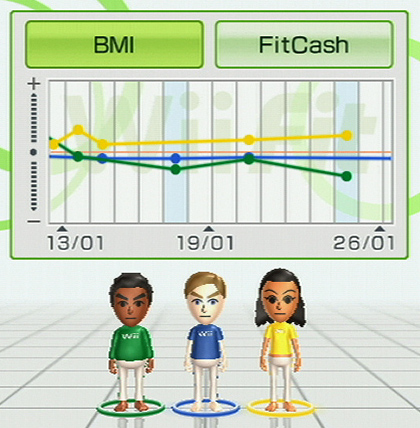
\includegraphics[width=0.5\linewidth]{images/wii_fit}
\caption{Courbes de progression au cours du temps dans le jeu Wii Fit.}
\label{fig:wii_fit}
\end{figure}

\begin{figure}[h!]
\centering
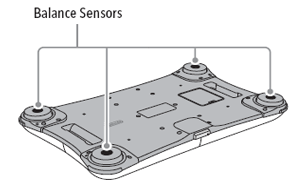
\includegraphics[width=0.5\linewidth]{images/balance_board}
\caption{La Wii Balance board de Nintendo.}
\label{fig:balance_board}
\end{figure}


\subsubsection{Nike+ Kinect Training}


% ------------------------------------------------------------------------------  

\subsection{Applications thérapeutiques}

\subsubsection{"Wiihabilitation"}

Les jeux Wii demandent souvent un mouvement du membre supérieur pour y 
jouer. De ce fait, de nombreuses 
cliniques aux États Unis se sont mis à les détourner à des buts 
thérapeutiques. Il s'agit bien ici de "détourner"~: rares sont les cas où des
applications spécifiques sont développées pour ce système par un tiers. Ceci
est probablement du au manque d'outils de développement officiels. Il existe
cependant un très grand nombre d'outils et de bibliothèques non-officiels, et
c'est d'ailleurs le succès de ces efforts qui a motivé Adafruit à offrir sa prime
pour l'ouverture de la Kinect.
% http://wiibrew.org/wiki/List_of_development_tools



%http://atwiki.assistivetech.net/index.php/Wii_rehab_applications_%28wiihab%29
%http://usatoday30.usatoday.com/tech/science/2008-02-08-wii-rehabilitation_N.htm

\subsubsection{MOJOS}
Lancé en 2010 avec un cycle de développment de 3 ans, 
La Moteur~de~Jeu~Orienté~Santé (MOJOS) est une collaboration entre~:
\begin{itemize}
\item \textbf{professionnels} de DIDACT Systèmes, NetDivision et GENIOUS,
\item \textbf{informaticiens} de l'UM2 et du LIRMM,
\item \textbf{médecins} de l'UM1, du CHU et du centre 
de recherche Efficience et Déficience Motrice (EDM),
\item \textbf{l'IDATE}, \emph{think tank} pour l'innovation numérique.
\end{itemize}

\paragraph{}
Son objectif était de développer un moteur de jeu permettant 
l'élaboration facile d'applications à but thérapeutiques, avec une étude 
expérimentale
par la suite, pour vérifier la pertinence de ces applications. En est sorti 
notamment le jeu Voracy Fish de GENIOUS (voir figure~\ref{fig:voracy_fish})
qui propose un exercice du membre supérieur~: le patient contrôle un poisson 
vorace grâce à une Kinect.

\begin{figure}[h!]
\centering
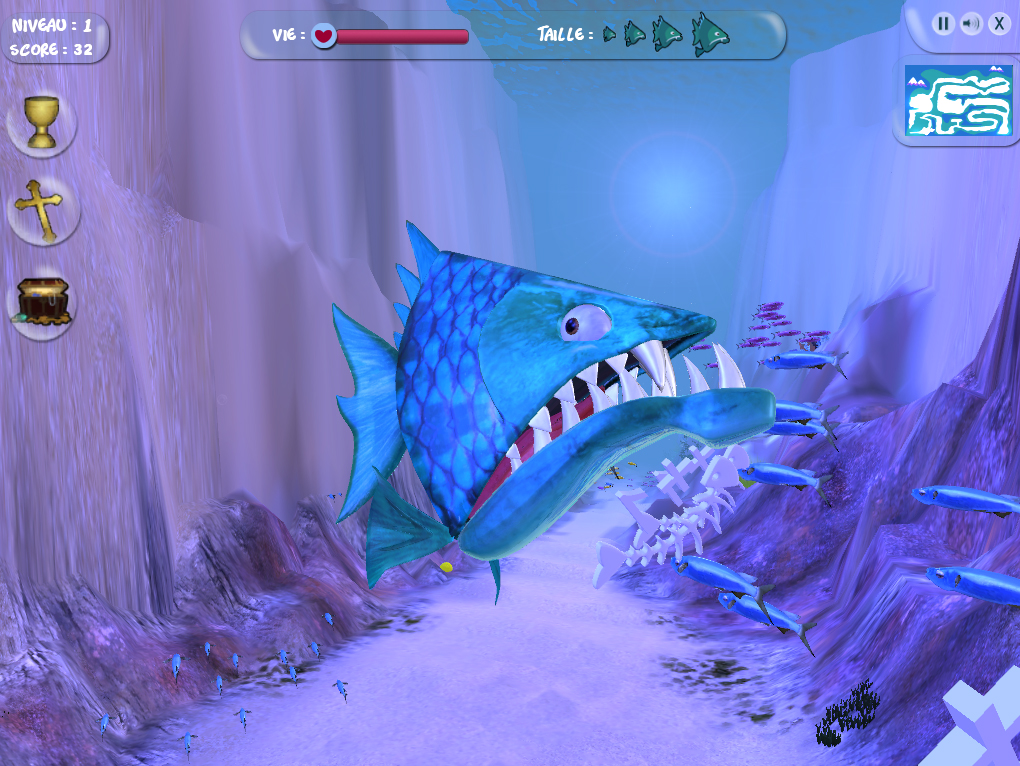
\includegraphics[width=0.8\linewidth]{images/voracy_fish}
\caption{Capture d'écran du jeu "Voracy Fish" de GENIOUS.}
\label{fig:voracy_fish}
\end{figure}

MOJOS se différencie d'un moteur jeu "normal" dans la mesure où 'il propose
un rééquilibrage dynamique de la difficulté afin de garder le patient dans
ce que Mihály Csíkszentmihályi nomme "Le Flux". Il y a en plus un suivie possible 
des performances du patient par son médecin.
% https://en.wikipedia.org/wiki/Flow_%28psychology%29

% http://www.mojos.fr/home/

\subsubsection{Hammer \& Planks}
Hammer \& Planks, jeu en développement par NaturalPad, se veut à la fois 
ludique et thérapeutique. Il est donc possible de contrôler le jeu via différents contrôleurs, dont une manette ou une Kinect.

\begin{figure}[h!]
\centering
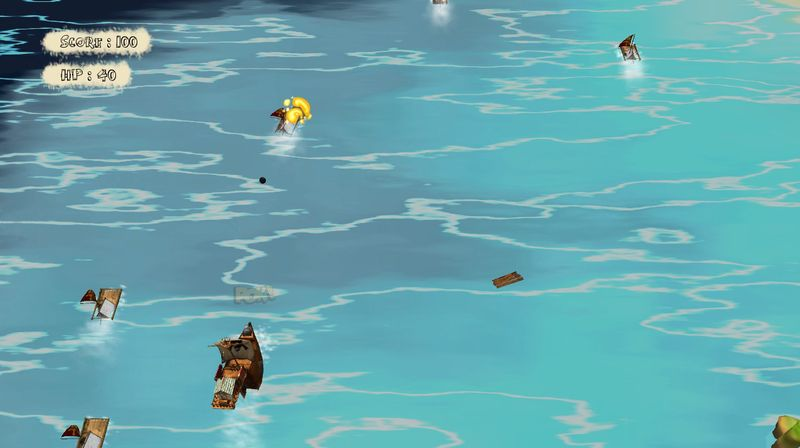
\includegraphics[width=1.0\linewidth]{images/hammer_and_planks}
\caption{Capture d'écran du jeu "Hammer and Planks" de 
NaturalPad.}
\end{figure}

Parmi les points intéressants il est offert ici la possibilité de modifier certains
paramètres du jeu par l'intermédiaire d'un terminal annexe, l'idée étant de
permettre à un spécialiste de rééquilibrer le jeu selon les besoins de son
patient.
